\documentclass{standalone}
\usepackage{xcolor-solarized}
\usepackage{tikz}
\usetikzlibrary{calc}
\usetikzlibrary{positioning}
\usetikzlibrary{arrows}
\usetikzlibrary{calc}
\usetikzlibrary{fit}
\usetikzlibrary{spy}
\usetikzlibrary{backgrounds}
\usetikzlibrary{shapes.symbols}

\begin{document}
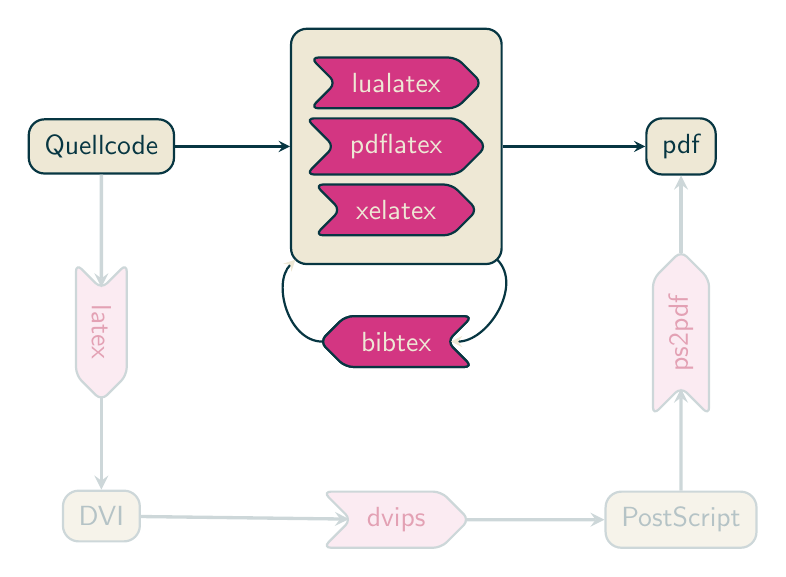
\begin{tikzpicture}[
    draw=solarized-base02,
    rounded corners=2mm,
    text=solarized-base02,
    every node/.append style={
        draw,
        thick,
        fill=solarized-base2,
        inner sep=2mm,
        font=\fontsize{10}{11}\selectfont,
        align=left,
    },
    signal/.append style={
        text=solarized-base2,
        fill=solarized-magenta,
        rounded corners=1mm,
    },
]
    \sffamily
    \node (source) 
        [align=left] 
        at (0,0)
        {Quellcode};

    \node (pdflatex) 
        [signal,shape=signal,signal from=west,signal to=east,right=20mm of source]
        {pdflatex};

    \node (pdf) 
        [right=20mm of pdflatex]
        {pdf};

    \begin{scope}[
        draw=solarized-base02!20!white,
        very thick,
        arrows={-{stealth[solarized-base02!20!white]}},
        rounded corners=2mm,
        text=solarized-base02!30!white,
        every node/.append style={
            draw,
            thick,
            fill=solarized-base2!50!white,
            inner sep=2mm,
            font=\fontsize{10}{11}\selectfont,
            align=left,
        },
        signal/.append style={
            text=solarized-base2!60!solarized-magenta,
            fill=solarized-magenta!10!white,
            rounded corners=1mm,
        },
    ]

        \node (latex) 
            [signal,shape = signal,signal from=west,signal to=east,
            below=of source,yshift=-10mm,rotate=-90,anchor=center] 
            {latex};

        \node (dvi) 
            [below=40 mm of source]
            {DVI};

        \node (dvips) 
            [signal,shape = signal,signal from=west
            ,signal to=east,below=40mm of pdflatex]
            {dvips};

        \node (postscript) 
            [below=40mm of pdf]
            {PostScript};

        \node (ps2pdf) 
            [signal,shape=signal,signal from=west,signal to=east,
            below=of pdf,yshift=-10mm,rotate=90,anchor=center]
            {ps2pdf};

    \end{scope}

    \begin{scope}[
            very thick,
            draw=solarized-base02!20!white,
            arrows={-{stealth[solarized-base02!20!white]}},
    ]
        \draw (source) -- (latex);
        \draw ($(latex.east) + (0,0.5mm)$) -- (dvi);
        \draw (dvi) -- (dvips);
        \draw ($(dvips.east) + (-0.5mm,0)$) -- (postscript);
        \draw (postscript) -- (ps2pdf);
        \draw ($(ps2pdf.east) + (0,-0.5mm)$) -- (pdf);
    \end{scope}

    % Additional Compilers, for the fitting node
    \node (xelatex) 
        [signal,shape = signal,signal from=west,
        signal to=east,below=1mm of pdflatex]
        {xelatex};

    \node (lualatex) 
        [signal,shape=signal,signal from=west,
        signal to=east,above=1mm of pdflatex] 
        {lualatex};

    \node (bibtex) 
        [signal,shape = signal,signal from=east,
        signal to=west,below=10mm of xelatex]
        {bibtex};

    % Using   the  'on   background  layer'  breaks  the
    % pre-pause slide, so we don't.
    \node (compilers) 
        [draw,fill=solarized-base2,fit=(lualatex) (pdflatex) (xelatex),
        inner sep=1em,xshift=-0.5em,align=right]
        {};

    % And  we  draw  this  stuff  twice,  so  that  it's
    % actually visible.
    \node (pdflatexTop) 
        [signal,shape = signal,signal from=west,
        signal to=east,right=20mm of source]
        {pdflatex};

    \node (xelatexTop) 
        [signal,shape = signal,signal from=west,
        signal to=east,below=1mm of pdflatex]
        {xelatex};

    \node (lualatexTop) 
        [signal,shape = signal,signal from=west,
        signal to=east,above=1mm of pdflatex]
        {lualatex};

    \node (bibtexTop) 
        [signal,shape = signal,signal from=east,
        signal to=west,below=10mm of xelatex]
        {bibtex};

    \draw ($(compilers.south east) + (-0.7mm,0.7mm)$)
        edge[thick,arrows={-{stealth[solarized-base2]}},out=-45,in=0] 
        ($(bibtex.east) + (0.3mm,0)$);
    \draw ($(bibtex.west) + (0.5mm,0)$)
        edge[thick,arrows={-{stealth[solarized-base2]}},out=180,in=225] 
        ($(compilers.south west) + (0.7mm,0.7mm)$);

    \begin{scope}[thick,arrows={-{stealth[solarized-base02]}}]
        \draw (source) -- (compilers.west);
        \draw (compilers.east) -- (pdf);
    \end{scope}
\end{tikzpicture}
\end{document}
